\documentclass[a4paper, 12pt, fleqn]{article}
\usepackage[czech]{babel}
\usepackage[utf8x]{inputenc}
\usepackage[T1]{fontenc}
%\usepackage[latin2]{inputenc} % pro iso8859-2
%\usepackage[IL2]{fontenc}     % fonty vygenerované pro iso8859-2

%%%%%%%%%%%%%%%%%%%%%%%%%%%%%%%%%%%%%%%%%%%%%%%%%%%%%%%%%%%%%%%%%%%%%%%%%
%% Hlavička ZDE VYPLNIT 
\newcommand{\autor}{Daniel KARLÍK, Michaela MAŠKOVÁ}
\newcommand{\cislomp}{2} % 1,2,3
\newcommand{\zadani}{Floor-field model se statickým polem}
\newcommand{\rocnik}{2020/2021}
%% Konec hlavičky
%%%%%%%%%%%%%%%%%%%%%%%%%%%%%%%%%%%%%%%%%%%%%%%%%%%%%%%%%%%%%%%%%%%%%%%%%


%\usepackage{enumitem} 
%\setlist{noitemsep, nolistsep}

\usepackage{calc}
\setlength{\textheight}{10in}
\setlength{\textwidth}{6.5in}
\setlength\oddsidemargin{0cm}
\setlength\evensidemargin{(0cm}
\setlength\topmargin{(\paperheight-\textheight-\headheight-\headsep-\footskip)/2 - 1in}

%% matematika
\usepackage{amssymb}
\usepackage{amsmath}

%% grafika
\usepackage{color}
\usepackage{tikz}
\usetikzlibrary{decorations.pathreplacing, patterns}
\usetikzlibrary{arrows.meta,positioning, datavisualization}
\usepackage{graphicx}
%\usepackage{animate}
\usepackage{booktabs}

%% plots
\usepackage{pgfplots}
\pgfplotsset{compat=1.16}
\usepackage{caption}
\usepackage{subcaption}

%% Nastavení grafiky matlabovských kódů ------------------------------------------------
\usepackage{verbatim}
\usepackage{listings} % balíček pro blok kódu
\usepackage{matlab-prettifier} % matlabovské barvičky atd.
\renewcommand{\lstlistingname}{Kód} % úprava caption
% nějaké další drobnosti
\lstset{basicstyle=\mlttfamily}
\lstset{frame=single}
\lstset{numbers=left}

% pro případ použití speciálních českých znaků v kódu (např. v komentáři)
\lstset{literate=
	{í}{{\'i}}1
	{á}{{\'a}}1
	{ý}{{\'y}}1
	{é}{{\'e}}1
	{ř}{{\v{r}}}1
	{ó}{{\'o}}1
	{ů}{{\r{u}}}1
	{č}{{\v{c}}}1
	{ě}{{\v{e}}}1
	{ž}{{\v{z}}}1
}



% ---------------------------------------------------------------------------------------
\begin{document}
	%%%%%%%%%%%%%%%%%%%%%%%%%%%%%%%%%%%%%%%%%%%%%%%%%%%%%%%%%%%%%%%%%%%%%%%%%%%%%%%%
	%% Vysázení hlavičky - NEMĚNIT
	\hrule
	\medskip
	\noindent{\Large \textbf{01SSI} -- Miniprojekt číslo \cislomp\hfill\rocnik}
	\hrule
	\medskip
	{\large
		\noindent
		\begin{tabular}{lp{12cm}}
			Posluchači:& \textbf{\autor}\\
			Zadání:& \textbf{\zadani} \\
		\end{tabular}
		
		\medskip
		\noindent
		\hspace{2mm}Odevzdáno: \hfill Získané body: \hfill Finální: ANO/NE
	}
	\medskip
	\hrule
	%% Konec vysázení hlavičky
	%%%%%%%%%%%%%%%%%%%%%%%%%%%%%%%%%%%%%%%%%%%%%%%%%%%%%%%%%%%%%%%%%%%%%%%%%%%%%%%%%%%%
	
	%% Vlastní popis
	
	\section{Teoretický úvod}
	\subsection{Celulární modely}
	
	Nejdříve si popíšeme proč je výhodné se \textit{celulárními modely} zabývat a jaké jsou jejich možné aplikace. Následně na to navážeme jejich formálním matematickým zavedením.
	
	Celulární modely nám umožňují popsat a studovat situace, kdy máme systém několika částic, které mají tendenci pohybovat se nějakým daným směrem a zároveň spolu interagují. Celulární modely se tedy sestávají z konfigurace poloh částic (pracujme např. s $ N $ částicemi) $ x = (x_{1}, \cdots, x_{N}) $ a interakcí, které jsou popsány potenciálem $ U(x) $.
	
	Tento typ modelů má široké spektrum využití, ať už ve studiu dopravních proudů nebo třeba jiných fyzikálních modelech. V historii se objevili i tací badatelé, kteří se zabývali filozofickými otázkami typu zda není i náš vesmír jistým celulárním systémem. Tyto otázky však přenecháme povolanějším a budeme se zabývat jednoduchými systémy.
	
	Důležitou součástí celulárních modelů je definice okolí buněk, jelikož se budeme zabývat buňkami ve 2D mřížce, tak si zadefinujeme okolí právě pro tyto případy.
	
	\textbf{Okolím buňky} $ x \in \mathbb{L} $, kde $\mathbb{L}$ značí množinu buněk,  budeme rozumět
	\begin{align}
	\mathsf{N}_{x} = {y \in \mathbb{L}: dist(x,y) \leq d }
	\end{align}
	
	% Nechceme matematicke "texty" psat v \mathsf{} ?
	
	Ve 2D tedy definujeme pro $ \forall x,y \in \mathbb{L}, x = (x_{1}, x_{2}), y = (y_{1}, y_{2}) $
	
	\textbf{Von Neumannovo okolí} jako výše zmíněné okolí v případě, kdy bereme 
	\begin{align}
	dist(x,y) = |x_{1} - y_{1}| + |x_{2} - y_{2}| \wedge d = 1 \label{VonNeumann}
	\end{align}
	
	\textbf{Moorovo okolí} bude okolí splňující následující
	\begin{align}
	dist(x,y) = max\{|x_{1} - y_{1}|,|x_{2} + y_{2}|\} \wedge d = 1 \label{Moor}
	\end{align}
	
	Obecně však může pohyb částic probíhat na nějaké množině buněk, reprezentované nějakým polem libovolné dimenze. Od tvaru této množiny se pak odvíjí možná volba okolí buněk. Zároveň zde vyvstává otázka, jak samotný pohyb částic probíhá.
	
	Podívejme se na to, jakým způsobem mohou být částice v množině buněk rozptýleny. Neboť chceme simulovat modely ve kterých neuvažujeme nehmotnost částic (uvažujeme např. chodce), pak se v jeden čas může v jedné buňce vyskytovat maximálně jedna částice. Tedy dostáváme množinu možných stavů $ \mathsf{S} = \{0, 1\} $ a stav buňky $ x \in \mathbb{L} $ splňuje následující vztah 
	\begin{equation}
	\tau(x)= \left \{
	\begin{aligned}
	&0, && x\text{ je prázdné} \\
	&1, && x\text{ je obsazené}
	\end{aligned} \right.
	\end{equation}
	
	Částice v modelu se vždy mohou pohybovat pouze do neobsazených buněk svého okolí nebo setrvat ve stávající buňce. Neboť budeme pracovat v diskrétním čase, pak připadá pohyb částice na jednu časovou jednotku. Pro naše účely budeme předpokládat, že $ v_{max} \leq 1 $, tzn. že se částice může pohnout za jednu časovou jednotku maximálně do okolní buňky, kdybychom ji volili vyšší pak by se náš model značně zkomplikoval.
	
	ZMÍNIT TASEP?
	
	Pohyb částic v modelu představuje změnu stavu modelu. Takovou změnu modelu budeme nazývat \textit{update}. Obecně je možné \textit{update} stavu systému rozdělit na dva typy. První představuje, tzv. \textit{paralelní update}, který představuje, že pohyb všech částic probíhá najednou. Druhý typ  můžeme nazývat např. \textit{postupný update} a označuje update ve kterém probíhá pohyb částic jednu po druhé. Takový pohyb probíhá podle nějak zvoleného pořadí. Užitím paralelního updatu může dojít ke konfliktu mezi částicemi a to takovému, že se více částic se chce přesunout do stejné buňky. To lze vyřešit tím, že náhodně vybereme jednu z částic, která se na onu buňku přesune.
	
	
	\subsection{Floor-field model}
	
	V této kapitole se blíže podíváme na tzv. \textit{Floor-field model}, jedná se o konkrétní typ modelu spadající do skupiny \textit{celulárních modelů}. 
	Vyznačuje se tím, že se jedná o model na dvoudimenzionální mřížce. Tuto dvoudimenzionální mřížku překryjeme polem, pomocí kterého budeme moci daný model dále studovat. 
	Pro \textit{Floor-field model} je obvyklé, že se pracuje s dvěma různými poli. První je tzv. \textit{statické} a druhé \textit{dynamické}. Statické pole představuje pole, které se vyčíslí na počátku daného pokusu a nadále nedochází k jeho změnám. Může se například jednat o vzdálenost od atraktoru, např. únikový východ pro evakuující. Oproti tomu dynamické pole se po každém proběhnuvším kroku musí aktualizovat, jako příklad můžeme uvést stopy označující cestu, kterou se vydal nějaký jedinec v minulosti. V takovém případě většinou platí jednoduchý vztah, čím čerstvější stopa tím silnější.
	
	Pravděpodobnost přechodu ze stavu systému $ x $ do stavu $ y $ označíme intuitivně $ P(x \rightarrow y) $. Bude pro ně platit vztah 
	\begin{align}
	\mathbb{P}(x \rightarrow y) \propto \exp\left\lbrace -\sum_{F}k_{F}F(y)\right\rbrace
	\label{Prechod}
	\end{align}
	kde $ F $ značí pole a $ k_{F} \in \langle 0, +\infty) $ je parametr.
	
	Statické pole budeme obecně značit $ S $. Hodnoty obsažené v polích závisí na zvoleném tvaru okolí buněk, pro naše účely postačí dvojice již dvě definovaná okolí \textbf{Von Neumannovo} (\ref{VonNeumann}) a \textbf{Moorovo} (\ref{Moor}).
	
	Máme-li floor-field model, ve kterém parametr $ k_{F} = k_{S} \rightarrow 0 $, pak pole statické pole $ S $ nehraje v modelu roli.  
	
	\subsection{Markovské procesy}
	
	Floor-field model lze modelovat také jako markovský proces. Mřížka, ve které se částice pohybuje, jsou jednotlivé stavy. Markovův řetězec definovaný nad touto mřížkou bude absorpční, neboť uvažujeme atraktor, který představuje právě absorpční stav.
	
	Pro Markovský proces lze sestavit tzv. matici pravděpodobností přechodu. Označíme-li $\tau_k$ stav v čase $k$, pak pro prvky matice přechodu $P$ platí:
	\begin{equation}
	[P]_{ij} = p_{ij} = \mathbb{P} [\tau_{k+1} = j | \tau_k = i],
	\end{equation}
	tedy jedná se o pravděpodobnost přechodu ze stavu $i$ do stavu $j$ v časovém skoku $k \rightarrow k + 1$. Budeme-li uvažovat, že $\tau_k$ odpovídá stavu $x$ a $\tau_{k+1}$ stavu $y$, definice splyne s \eqref{Prechod}.
	
	Jistě platí, že pro $i$ absorpční stav je $[P]_{ii} = 1$ a $[P]_{ij} = 0 \quad \forall j \neq i$, částice tedy nemůže přeskočit do jiného stavu a zůstává ve stavu $i$. Budeme-li uvažovat místnost s překážkami, pak překážka je také absorpčním stavem ozn. $z$, tedy $\mathbb{P}[z \rightarrow z] = 1$, do kterého ale není možné přejít, takže
	\[
	\mathbb{P}[z \rightarrow x] = 0 \quad \land \quad \mathbb{P}[x \rightarrow z] = 0 \quad  \forall x \neq z.
	\]
	
	Jelikož se ve floor-field modelu pohybujeme na 2D mřížce, zavedeme následující indexování: pro 2D mřížku rozměru $n \times n$ dostaneme $n^2$ stavů. Stav $k \in \{1,2,\dots,n^2\}$ bude po řadě odpovídat souřadnicím $(i,j) \in \{ (1,1),(2,1),(3,1),\dots,(n-2,n),(n-1,n),(n,n) \}$. Příkladem může být následující matice stavů
	\begin{equation*}
	\begin{pmatrix}
	1 & 4 & 7 \\
	2 & 5 & 8 \\
	3 & 6 & 9 \\
	\end{pmatrix},
	\end{equation*}
	kde mřížka je velikosti $3 \times 3$ a má tedy 9 stavů.
	
	V rámci protokolu budeme chtít sledovat \textbf{střední dobu do pohlcení}, která je definována jako
	\begin{equation}
	h_A(k) = \mathbb{E} \left[ T_A | \tau_0 = k \right],
	\end{equation}
	kde $A$ představuje množinu absorpčních stavů a $k$ je počáteční stav, $S$ je množina všech stavů. Tato podmínka lze dále přepsat jako
	\begin{equation}
	h_A(k) = 1 + \sum_{l \in S \setminus A} P_{kl} h_A(l), \quad k \in S \setminus A.
	\end{equation}
	
	Zjednodušení představuje, pokud můžeme matici $P$ napsat ve tvaru
	\begin{equation}
	\begin{pmatrix}
	\mathbb{Q} & \mathbb{R} \\
	\mathbf{0} & \mathbb{I}_r
	\end{pmatrix},
	\label{Eq: FundMat}
	\end{equation}
	kde $\mathbb{Q}$ je $t \times t$ matice, $\mathbb{R}$ je $t \times r$ matice, $\mathbf{0}$ je nulová $r \times \r$ matice a $\mathbb{I}_r$ je identická matice velikosti $r \times r$. Pak můžeme sestavit tzv. fundamentální matici $\mathbb{N}$, pro kterou platí
	\begin{equation}
	\mathbb{N} = \sum_{k=0}^{\infty} \mathbb{Q}^k = \left( \textbb{I}_r - \mathbb{Q} \right)^_{-1}.
	\label{Eq: N}
	\end{equation}
	Střední doba do pohlcení lze pak spočítat jako
	\begin{equation}
	\mathbf{t} = \mathbb{N} \mathbf{1},
	\label{Eq: Vypocet Et}
	\end{equation}
	což nám dá vektor těchto středních dob pro všechny tranzientní stavy.
	
	\section{Kód}
	
	Pro běh simulace bylo třeba vytvořit několik pomocných funkcí, které umožnily například najít souřadnice buněk v Neumannově okolí referenční buňky, vypočítat statické pole apod. Byla použita mřížková metrika $\mathrm{dist}(x,y) = |x_1 - x_2| + |y_1 - y_2|$.
	
	Pro simulaci byla vytvořena dvě pole jako matice. Matice \verb|pole| v sobě uchovává informaci o překážkách ($-1$), částicích ($+1$) a volných buňkách ($0$). Matice \verb|staticke_pole| pak uchovává informaci o překážkách a ve zbylých políčkách jsou hodnoty představující vzdálenost daného políčka od atraktoru.
	
	\subsection{Funkce pro simulaci pohybu v mřížce}
	Funkce \verb|dist| definuje vzdálenost mezi dvěmi buňkami. Funkce \verb|neumann_okoli| pak vrací hodnotu \verb|true| v případě, že se buňka nachází v Neumannově okolí referenční buňky a \verb|false| v opačném případě.
	
	\begin{lstlisting}[language=Matlab]
	function dist(b1, b2)
	x1, y1 = b1
	x2, y2 = b2
	abs(x1 - x2) + abs(y1 - y2)
	end
	
	function neumann_okoli(b1, b2)
	dist(b1, b2) == 1
	end
	\end{lstlisting}
	
	Následují funkce pro vyplnění statického pole vzdálenostmi od atraktoru. Funkce \linebreak \verb|dist_pole(pole,b)| vytvoří \uv{masku}, která nám označí hodnotou \verb|true| ty prvky matice, které jsou v Neumannově okolí buňky $b$. Funkce \verb|update_pole(pole,b,max_value)| pak tuto masku použije k přičení $1$ do statického pole na správném místě. Obě funkce jsou iterativně použity v poslední funkci \verb|spocitej_S|, která pomocí \verb|while| cyklu iterativně vyplňuje statické pole, dokud není zcela zaplněno.
	
	\begin{lstlisting}[language=Matlab]
	function dist_pole(pole, b)
	max_value = maximum(pole)
	tmp = zeros(n, n)
	for x in 1:n
	for y in 1:n
	if neumann_okoli((x, y), b) && (pole[x,y] == 0)
	tmp[x,y] = 1
	end
	end
	end
	mask = tmp .== 1
	end
	
	function update_pole(pole, b, max_value)
	mask = dist_pole(pole, b)
	pole[mask] .= max_value + 1
	return pole
	end
	
	function spocitej_S(pole, atraktor)
	max_value = maximum(pole)
	update_pole(pole, atraktor, max_value)
	while sum(pole .== 0) > 0
	max_value = maximum(pole)
	indexes = findall(x -> x == max_value, pole)
	
	for b in Tuple.(indexes)
	update_pole(pole, b, max_value)
	end
	end
	end
	\end{lstlisting}
	
	Tím jsme schopní spočítat statické pole. Teď už potřebujeme jen novou pozici částic v našem systému. Částice přeskočí do políčka ve svém okolí s pravděpodobností definovanou vztahem \eqref{Prechod}. Funkce \verb|preskok(pole,ks)| nejdříve najde souřadnici, kde se nachází částice. Pak vytvoří masku Neumannova okolí této částice. Zjistí si hodnotu statického pole v těchto buňkách a přidá hodnotu statického pole i buňky, ve které se částice právě nachází. Podle vzorce \eqref{Prechod} jsou spočítány pravděpodobnosti přechodu do daných buněk. Následně je náhodně vybrán index z kategorického rozdělení se získaným pravděpodobnostním vektorem. Posledním krokem je získat souřadnice vybrané buňky pro přeskok a provést update pole.
	
	\begin{lstlisting}[language=Matlab]
	function preskok(pole,ks)
	b_idx = findall(x -> x == 1, pole)[1]
	mask = dist_pole(pole, Tuple(b_idx)) 
	vec_S = staticke_pole[mask]          
	idx_mask = findall(x -> x == 1, mask)
	idx_mask = vcat(idx_mask, b_idx)     
	vec_S = vcat(vec_S, staticke_pole[b_idx]) 
	
	jmenovatel = sum(exp.(.- vec_S .* ks))
	P_ks = exp.(.- vec_S * ks) ./ jmenovatel
	idx = rand(Categorical(P_ks))
	
	idx_skok = idx_mask[idx]                  
	pole[b_idx] = 0
	pole[idx_skok] = 1
	end
	\end{lstlisting}
	
	Pro více částic v poli fungují funkce velmi podobně. Možné konflikty při skoku více částic, které mohou skočit do stejného pole, byly vyřešeny jednoduše. Update byl proveden iterativně postupně pro každou částici zvlášť. Není tak nutno konflikty řešit. Jedná se samozřejmě o jisté zjednodušení podobné například situaci, kdy funguje tzv. přednost zprava. Nicméně domníváme se, že toho zjednodušení nevnese do řešeného případu velký problém.
	
	Další funkce už jsou jen pomocné funkce pro grafické znázornění výsledků a provedení samotné simulace a není třeba je zde zmiňovat.
	
	\subsection{Matice přechodu}
	
	Pro získání matice přechodu bylo vytvořeno ještě jedno pomocné pole nazvané \verb|pole_bezcastic|. Toto pole obsahuje pouze 0, jedná-li se o obyčejné políčko, kam mohou skákat částice, a 1, pokud se zde nachází překážka nebo se jedná o pozici atraktoru.
	
	Výpočet matice pak probíhá iterativně velmi podobně jako ve funkci \verb|preskok|. Pro každé políčko v mřížce je spočítán vektor pravděpodobností přechodu z tohoto políčka do jiného. Pro překážky je vektor naplněn nulami a jedničkou v místě překážky, stejně tak pro atraktor.
	\pagebreak
	\begin{lstlisting}[language=Matlab]
	function matice_prechodu(pole_bezcastic, staticke_pole, ks)
	# inicializace prázdné matice přechodu
	P = zeros(n*n,n*n)
	i = 1
	# smyčka pro výpočet jednotlivých řádků P
	for b_idx in findall(x -> x == 1, ones(5,5))
	# pokud překážka nebo atraktor
	if pole_bezcastic[b_idx] == 1
	pravd_prechodu = zeros(5,5)
	pravd_prechodu[b_idx] = 1
	
	pvec = reshape(pravd_prechodu,1,:)
	P[i,:] .= pvec[:]
	# pokud klasické pole
	else
	mask = dist_pole(pole, Tuple(b_idx))                    
	mask[b_idx] = 1                                         
	vec_S = staticke_pole[mask]                             
	idx_mask = findall(x -> x == 1, mask)                   
	
	jmenovatel = sum(exp.(.- vec_S .* ks))
	P_ks = exp.(.- vec_S * ks) ./ jmenovatel
	
	pravd_prechodu = zeros(5,5)
	pravd_prechodu[idx_mask] .= P_ks
	pvec = reshape(pravd_prechodu,1,:)
	
	P[i,:] .= pvec[:]
	end
	i += 1
	end
	return P
	end
	\end{lstlisting}
	
	Matice je dále upravena do požadovaného tvaru a je s ní dále manipulováno. Nicméně jako v předchozí sekci se jedná o funkce spíše nezajímavé a nebudeme je zde uvádět.
	
	\newpage
	\section{Simulace}
	
	\subsection{Mřížka $15 \times 15$}
	
	Pro větší mřížku byly vytvořeny simulace, které měly za cíl vizualizovat hustotu v $(i,j)$-té buňce pole, tedy bylo zkoumáno, kde se nejčastěji částice pohybovaly. Tato hustota byla následně vykreslena jako \textit{heatmap}, tedy mřížka, kde je barvou vyznačena hustota v dané buňce. Zkoumána byla závislost hustoty i na hodnotě konstanty $k_S$, která významně ovlivňuje chování částic.
	
	Zkoumaná mřížka měla rozměry $15 \times 15$ a simulace byla provedena pro 15 částic seřazených v řadě na jednom konci \uv{místnosti}. Ukázku mřížky s částicemi a překážkami lze vidět na Obr. \ref{Obr: Místnost}.
	
	\begin{figure}[h]
		\centering
		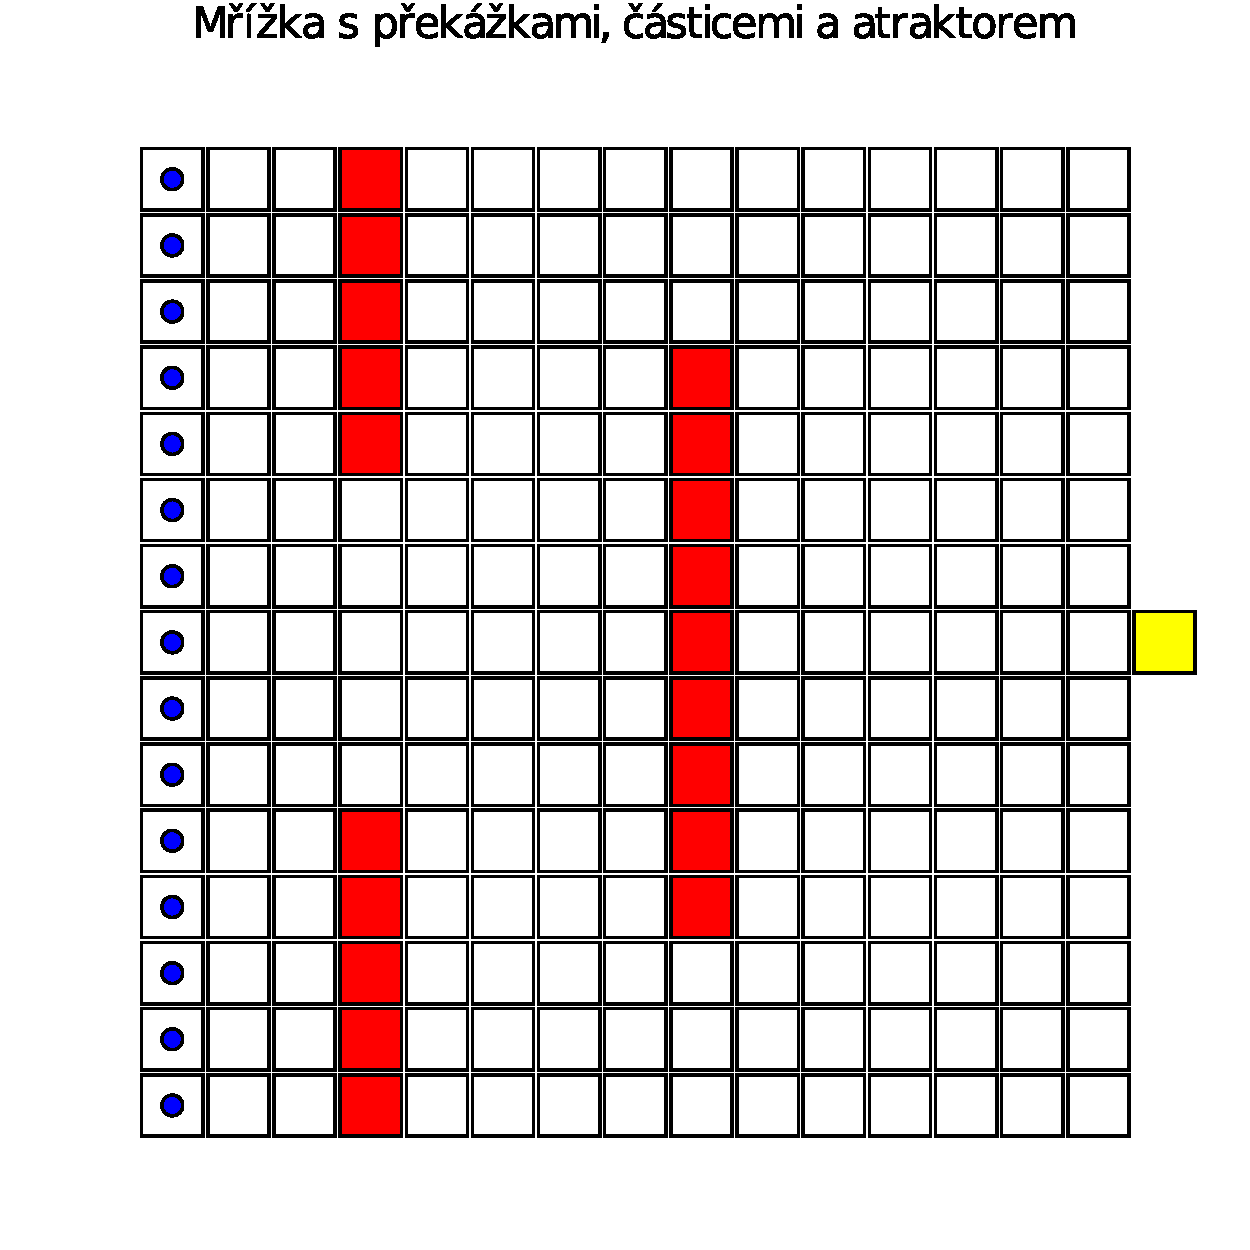
\includegraphics[trim={0 1cm 0 1cm},clip,width=0.8\linewidth]{images/mrizka.pdf}
		\caption{Mřížka použitá pro simulaci.}
		\label{Obr: Místnost}
	\end{figure}
	
	Je vidět, že mřížka je symetrická. Na obrázku \ref{Obr: Statické pole} lze dále vidět vykreslené statické pole, tedy jednotlivá políčka jsou znázorněná barevně podle toho, jak daleko jsou od atraktoru. Černou barvou jsou zvýrazněné i překážky.
	
	\begin{figure}
		\centering
		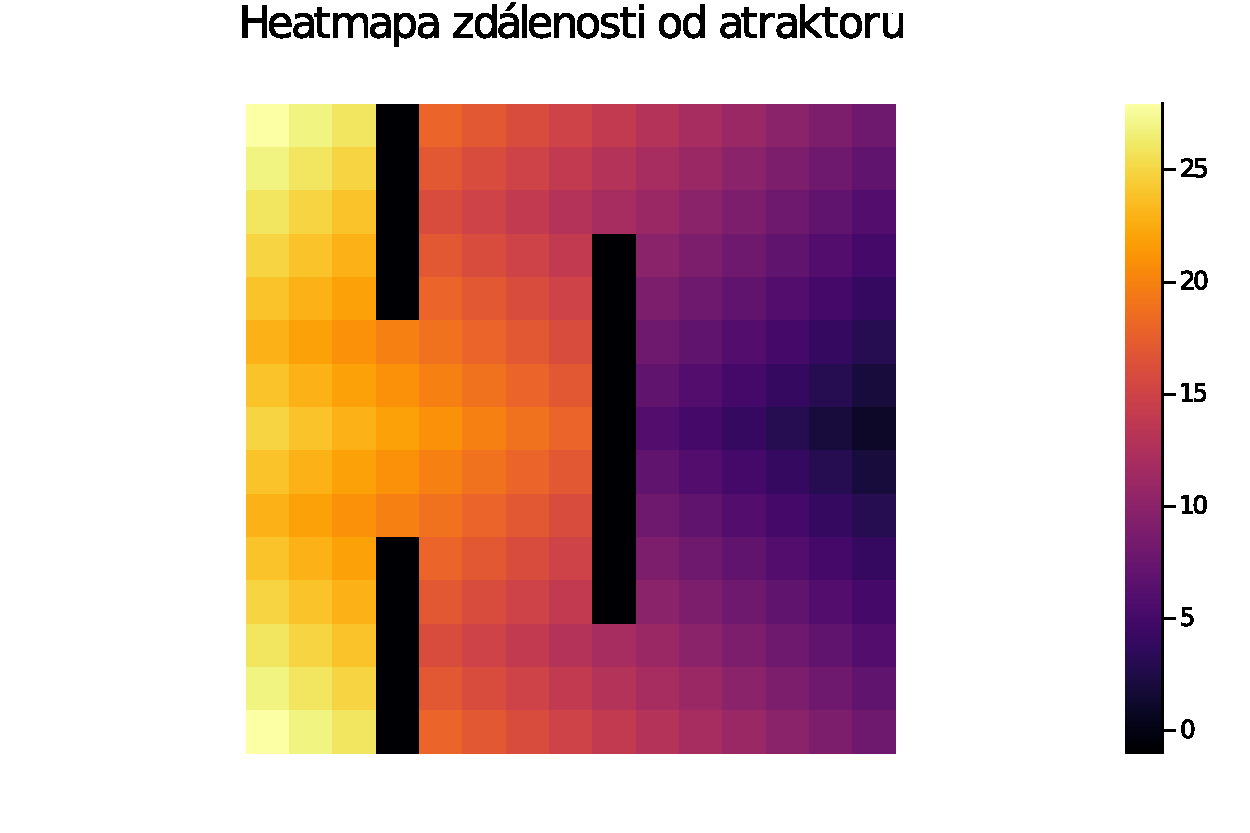
\includegraphics[width=\linewidth]{images/stat_pole.pdf}
		\caption{Heatmap vzdáleností od atraktoru -- vizualizace statického pole.}
		\label{Obr: Statické pole}
	\end{figure}
	
	Stejnou heatmapu můžeme vidět i pro místnost bez překážek na Obr. \ref{Obr: Statické pole bez překážek}.
	
	\begin{figure}
		\centering
		\includegraphics[width=\linewidth]{images/stat_pole_bezprekazek.pdf}
		\caption{Heatmap vzdáleností od atraktoru -- vizualizace statického pole.}
		\label{Obr: Statické pole bez překážek}
	\end{figure}
	\pagebreak
	\subsection{Mřížka $5 \times 5$}
	
	Pro sledování střední doby do absorpce byla vytvořena menší místnost velikosti $5 \times 5$, kterou lze vidět na Obr. \ref{Obr: Menší}. Ačkoli atraktor je zobrazen mimo mřížku, absorpčním stavem je ten, který má od atraktoru vzdálenost 1, tedy na obrázku stav v horním pravém rohu.
	
	\begin{figure}[h]
		\centering
		\includegraphics[trim={0 2cm 0 3cm},clip,width=0.7\linewidth]{images/mensi.pdf}
		\caption{Mřížka použitá pro simulaci -- menší.}
		\label{Obr: Menší}
	\end{figure}
	
	Pro různé hodnoty $k_S$ byla sledována střední doba do absorpce, aby bylo možné tuto dobu porovnat s teoretickými hodnotami. Jelikož mřížka je rozměrů $5 \times 5$, nachází se na ní celkem 25 stavů, proto bude mít matice pravděpodobností přechodu rozměry $25 \times 25$.
	
	\section{Výsledky}
	
	Tato sekce shrnuje do několika podsekcí výsledky získané v průběhu experimentu. Zaměřujeme se na střední dobu do pohlcení a průměrnou hustotu buněk v mřížce. Porovnáváme pro mřížku s překážkami i bez překážek, uvažujeme vliv konstanty $k_S$.
	
	Doporučujeme podívat se i na .gif soubory, které vizualizují jednotlivé simulace jako animace.
	
	\subsection{Střední doba do pohlcení}
	
	Pro samotnou částici byla řešena střední doba do pohlcení pro různé hodnoty konstanty $k_S$. Byla vybrána konfigurace jako na Obr. \ref{Obr: Menší}, tedy sledovala se střední doba absorpce ze stavu $(1,1)$ (resp. 1) do $(5,5)$ (resp. 25).
	
	\subsubsection{Simulace}
	
	Simulace byla provedena pro hodnoty $k_S \in \{0.001,0.005,0.01,0.05,0.1,0.2,\dots,2.9,3\}$. Pro každou hodnotu $k_S$ byla simulace spuštěna 30krát, následně byl spočítán průměr.
	
	Už předem můžeme o průběhu $k_S$ říct například to, že hodnota $\mathbb{E}\left[t_e \right]$ bude zdola omezena hodnotou statického pole v místě startu částice. Pokud totiž v každém čase může částice skočit o jedno políčko, bude minimální čas potřebný k dosažení atraktoru roven vzdálenosti od atraktoru. Pro $k_S \rightarrow \infty$ bude pravděpodobnost přechodu do buňky s nižší hodnotou statického pole $\rightarrow 1$.
	
	\subsubsection{Teoretický výsledek}
	
	Pro porovnání byla spočítána i teoretická hodnota střední doby do absorpce ze stavu $(1,1)$ do $(5,5)$. Pro stejné hodnoty $k_S$ jako v simulaci byla spočítána matice přechodu pravděpodobností $P$, kterou bylo dále třeba transformovat do tvaru \eqref{Eq: FundMat}. Následně stačilo využít vzorců \eqref{Eq: N} a \eqref{Eq: Vypocet Et} a spočítat střední dobu do absorpce pro hledaný stav.
	
	Pro ukázku můžeme na obrázcích  vidět heatmapu matic pravděpodobností přechodu opět pro různé hodnoty konstanty $k_S$. Obecně vidíme, že možností přechodu mnoho není, což je dáno faktem, že částice může přeskočit pouze ve svém Neumannově okolí. Nicméně se zvyšující se hodnotou $k_S$ můžeme sledovat, že pravděpodobnosti přechodu do stavu s nižší hodnotou statického pole jsou stále vyšší.
	
	\begin{figure}[h]
		\centering
		\includegraphics[width=0.7\linewidth]{images/P_0.pdf}
		\caption{Heatmap matice pravděpodobností přechodu pro $k_S = 0$.}
		\label{Obr: P0}
	\end{figure}
	
	\begin{figure}
		\centering
		\includegraphics[width=0.7\linewidth]{images/P_05.pdf}
		\caption{Heatmap matice pravděpodobností přechodu pro $k_S = 0.5$.}
		\label{Obr: P05}
	\end{figure}
	
	\begin{figure}
		\centering
		\includegraphics[width=0.7\linewidth]{images/P_1.pdf}
		\caption{Heatmap matice pravděpodobností přechodu pro $k_S = 1$.}
		\label{Obr: P1}
	\end{figure}
	
	\begin{figure}
		\centering
		\includegraphics[width=0.7\linewidth]{images/P_3.pdf}
		\caption{Heatmap matice pravděpodobností přechodu pro $k_S = 3$.}
		\label{Obr: P3}
	\end{figure}
	
	\pagebreak
	\subsubsection{Porovnání výsledků}
	
	Výsledné hodnoty jsou graficky znázorněné na Obr. \ref{Obr: MAT}.  Můžeme si všimnout, že simulace velmi dobře napodobuje trend daný teoretickou závislostí. Odchylky od teoretických hodnot se objevují hlavně pro $k_S < 1$. To je pravděpodobně způsobeno i tím, že průměr není robustní funkce a simulací pro každou hodnotu $k_S$ bylo provedeno 30. Vyšší počet simulací by mohl vést k přesnějším výsledkům.
	
	Nasimulované i teoretické hodnoty byly nafitovány funkcí
	\[ f(x) = a + b \exp(-cx). \]
	Pro porovnání jsou hodnoty koeficientů uvedené v tabulce \ref{Tab: koeficienty}.
	
	\begin{table}[h]
		\centering
		\begin{tabular}{rrrr}
			\toprule
			& a & b & c  \\ \toprule
			teorie & 9.9 & 80.3 & 3.9 \\ \midrule
			simulace & 11.2 & 84.0 & 3.9 \\ \bottomrule
		\end{tabular}
		\caption{Tabulka koeficientů nafitovaných na exponenciální funkci.}
		\label{Tab: koeficienty}
	\end{table}
	
	\begin{figure}
		\centering
		\includegraphics[width=0.9\linewidth]{images/stredni.pdf}
		\caption{Střední doba do absorpce -- porovnání nasimulovaných a teoretických hodnot.}
		\label{Obr: MAT}
	\end{figure}
	
	\pagebreak
	\subsection{Výsledky pro více částic}
	
	V modelu s více částicemi lze přepokládat, že interakce jednotlivých částic (zde fakt, že dvě částice nemohou být v jednu chvíli ve stejném poli mřížky) bude mít vliv na různé sledované veličiny. Například střední doba do pohlcení bude jistě delší, pokud budeme počítat dobu do pohlcení všech částic.
	
	\subsubsection{Hustota buněk}
	
	Nejdříve se podíváme na situaci, kdy neuvažujeme v místnosti žádné překážky.
	
	Průměrná hustota v buňkách byla sledována pro čtyři hodnoty konstanty $k_s \in \{0,0.5,1,3\}$. V prvním případě částice netuší, kterým směrem by se měly pohybovat a vzdálenost od atraktoru je pro ně bezvýznamná. To vidíme krásně i na hustotách pravděpodobnosti na Obr. \ref{Obr: Heatmap bez ks=0}. Tato konkrétní simulace byla provedena pro 1000 překoků, kdy ani poté nedosáhly všechny částice atraktoru a východu. Částice mají stejnou pravděpodobnost přeskoku do všech buněk ve svém okolí. Ve výsledku tak velmi často oscilují a nesledují žádný směr.
	
	\begin{figure}
		\centering
		\includegraphics[width=\linewidth]{images/heatmap_bezprekazek_ks=0.pdf}
		\caption{Heatmap hustoty v jednotlivých buňkách pro $k_S = 0$, mřížka bez překážek.}
		\label{Obr: Heatmap bez ks=0}
	\end{figure}
	
	Pro zbylé hodnoty konstanty $k_S$ už je situace lepší. Všechny částice se k atraktoru dostaly dříve než za $T = 100$ sekund. Na obrázcích \ref{Obr: Heatmap bez ks=0.5}, \ref{Obr: Heatmap bez ks=1} a \ref{Obr: Heatmap bez ks=3} můžeme postupně sledovat, že zvyšování kosntanty $k_S$ zvyšuje hustotu pravděpodobnosti, že se částice budou nacházet ve středu mřížky a budou se pohybovat co nejefektivněji směrem k atraktoru.
	
	\begin{figure}
		\centering
		\includegraphics[width=\linewidth]{images/heatmap_bezprekazek_ks=05.pdf}
		\caption{Heatmap hustoty v jednotlivých buňkách pro $k_S = 0.5$, mřížka bez překážek.}
		\label{Obr: Heatmap bez ks=0.5}
	\end{figure}
	
	\begin{figure}
		\centering
		\includegraphics[width=\linewidth]{images/heatmap_bezprekazek_ks=1.pdf}
		\caption{Heatmap hustoty v jednotlivých buňkách pro $k_S = 1$, mřížka bez překážek.}
		\label{Obr: Heatmap bez ks=1}
	\end{figure}
	
	\begin{figure}
		\centering
		\includegraphics[width=\linewidth]{images/heatmap_bezprekazek_ks=3.pdf}
		\caption{Heatmap hustoty v jednotlivých buňkách pro $k_S = 3$, mřížka bez překážek.}
		\label{Obr: Heatmap bez ks=3}
	\end{figure}
	
	Teď se přesuneme k případu, kdy už uvažujeme překážky jako v Obr. \ref{Obr: Místnost}. Opět uvažujeme stejné hodnoty konstany $k_S$ jako v předchozím případě: $(0,0.5,1,3)$. Na heatmapách jsou překážky znázorněny hodnotou $-0.05$, aby bylo barevně jasné, kde se nachází.
	
	Simulace pro $k_S = 0$ byla opět provedena pouze pro 1000 iterací, jelikož ani po takovém čase se částice nedokázaly dostat k atraktoru.
	
	\begin{figure}
		\centering
		\includegraphics[width=\linewidth]{images/heatmap_ks=0.pdf}
		\caption{Heatmap hustoty v jednotlivých buňkách pro $k_S = 0$, mřížka s překážkami.}
		\label{Obr: Heatmap ks=0}
	\end{figure}
	
	Na dalších obrázcích vidíme, jak se s roustoucí hodnotou $k_S$ měnil průběh hustoty. Částice si postupně hledají lepší a lepší cesty, už tolik neutíkají špatným směrem a rychleji se dokáží dostat k atraktoru.
	
	\begin{figure}
		\centering
		\includegraphics[width=\linewidth]{images/heatmap_ks=05.pdf}
		\caption{Heatmap hustoty v jednotlivých buňkách pro $k_S = 0.5$, mřížka s překážkami.}
		\label{Obr: Heatmap ks=0.5}
	\end{figure}
	
	\begin{figure}
		\centering
		\includegraphics[width=\linewidth]{images/heatmap_ks=1.pdf}
		\caption{Heatmap hustoty v jednotlivých buňkách pro $k_S = 1$, mřížka s překážkami.}
		\label{Obr: Heatmap ks=1}
	\end{figure}
	
	\begin{figure}
		\centering
		\includegraphics[width=\linewidth]{images/heatmap_ks=3.pdf}
		\caption{Heatmap hustoty v jednotlivých buňkách pro $k_S = 3$, mřížka s překážkami.}
		\label{Obr: Heatmap ks=3}
	\end{figure}
	
	\section{Závěr}
	
	V protokolu byl zkoumán floor-field model se statickým polem. Byla zkoumána hlavně závislost veličin jako je střední doba do pohlcení a hustota buněk v mřížce na hodnotě konstanty $k_S$. Experimentálně bylo potvrzeno, že zvyšující hodnota $k_S$ má za následek zrychlení pohybu částic a jejich rychlejší pohlcení.
	
\end{document}
